% Contenido del CursoICE_2024
\chapter{Pensar de manera funcional. Programación declarativa}
\label{ch_intro}

\IndiceCapitulo
\begin{Resumen}
   Se considera que la programación funcional está basada en el \textit{cálculo lambda},  un sistema formal desarrollado en los años 1930 para investigar la naturaleza de las funciones, de la computabilidad y su relación con la recursión. 
   
   \smallskip
   
   El objetivo de este curso es explicar las técnicas y la forma funcional de razonar en programación para mejorar la calidad del código de los programas.
\end{Resumen}

\section{¿En qué consiste la programación funcional?}
Es difícil definir el concepto de \textit{Programación Funcional} (PF). Se considera que la PF está incluida en el paradigma de la \textit{programación declarativa}, en la cual los lenguajes se centran en describir qué quieren hacer en lugar de detallar cómo hacerlo, como sucede en los lenguajes imperativos.

Los siguientes elementos formarían parte del conjunto de componentes que utilizan los lenguajes funcionales:

\begin{itemize}
   \item \textbf{Funciones puras:} se dice que una función es \textit{pura} si no produce efectos secundarios, no depende de ningún estado exterior y siempre proporciona el mismo resultado para el mismo valor de los argumentos de entrada. Se entiende por \textit{efecto secundario} cualquier acción del programa que no sea un cálculo. Por ejemplo, modificar el estado de una variable, mostrar un mensaje en una pantalla o enviar un correo electrónico serían ejemplos de efectos secundarios.
   \item \textbf{Funciones de orden superior:} las funciones que operan utilizando otras funciones se denominan \textit{funciones de orden superior}. En la programación funcional, las funciones se consideran \textit{elementos de primera clase}, lo que significa que se pueden tratar como cualquier otro tipo de datos: se pueden utilizar como parámetros o como valor devuelto por otras funciones y pueden asignarse a variables. En la mayoría de lenguajes hay elementos que no son de primera clase, por ejemplo los operadores o las cláusulas que definen los bucles o las bifurcaciones.
   \item \textbf{Closures:} en programación funcional es habitual utilizar un tipo especial de funciones denominadas \textit{closures}. Se trata de funciones anónimas definidas in situ que son capaces de capturar el entorno en el que fueron definidas, de forma que pueden acceder con posterioridad a variables de ese entorno con los valores que tuvieran en el momento en el que se declaró la \textit{closure}. Actualmente, las \textit{closures} también se incluyen en numerosos lenguajes, a veces bajo la denominación de \textit{funciones anónimas}.
   \item \textbf{Inmutabilidad de las variables:} la programación funcional pone especial énfasis en la utilización de estructuras \textit{inmutables}. Cambiar el valor de una variable, cambiar su estado, se considera un efecto secundario que hay que tratar de evitar. Decir que las \textit{variables} no deben variar puede parecer un contrasentido, pero no es un asunto excepcional en los lenguajes de programación. Por poner un ejemplo, en Java o en Javascript, las variables del tipo \textit{String} son inmutables. Cuando se quiere modificar el estado de una variable inmutable lo que se hace es crear una nueva variable con el nuevo valor. El procedimiento consiste en \textit{transformar} una variable en otra, en vez de en modificar el estado de la variable original. La inmutabilidad facilita los test de los programas y hace más segura la utilización de la programación multiproceso o en paralelo.
   \item \textbf{Recursividad:} el control de flujo en la programación funcional favorece la recursividad frente a los bucles. Sustituyendo los bucles del tipo \textit{for} o \textit{while} mediante recursividad se consigue un código más declarativo y, en ocasiones, más elegante.
   \item \textbf{Iteradores:} los \textit{iteradores} son una construcción habitual en la programación funcional y que, a día de hoy, incorporan muchos lenguajes. Son estructuras que permiten recorrer una colección de manera ordenada, sin recurrir a bucles y variables de índice. 
   \item \textbf{Evaluación perezosa:} las expresiones, siempre que se pueda, se deben comportar de manera \textit{perezosa}. La \textit{evaluación perezosa} (\textit{lazy evaluation}) consiste en que determinados cálculos que impliquen a variables no se realicen hasta que son estrictamente necesarios.
   \item \textbf{Sin estado ni efectos secundarios:} en la programación funcional se trata de minimizar los estados mutables y los efectos secundarios. El resultado es un código en el que es más fácil razonar, hacer test y realizar la depuración de errores. Cuando es necesario mantener estados o realizar acciones con efectos secundarios, se controla rigurosamente.
\end{itemize}

Tras leer los párrafos anteriores, el lector puede estar preguntándose cómo es posible realizar un programa de aplicación práctica sin efectos secundarios y sin cambiar el valor de las variables. Bien, no es posible, los programadores funcionales utilizan funciones impuras en numerosas ocasiones y necesitan utilizar variables mutables en determinados contextos. No obstante, durante el desarrollo de un programa, hay numerosas situaciones en las que la utilización de funciones puras y el respeto a la inmutabilidad proporciona más seguridad y da lugar a que el código generado sea más escalable.

La programación funcional no es una sintaxis determinada, consiste en una serie de técnicas orientadas a eliminar los efectos secundarios o, al menos, limitar su alcance. Si se utilizan estas técnicas de manera adecuada, se consigue escribir código más fácil de leer, más correcto, más seguro, más fácil de probar y más fácil de depurar, lo que a fin de cuentas es el objetivo fundamental que se debe perseguir al programar. 

La técnicas de la programación funcional no están restringidas por el lenguaje de programación que se utilice. Los conceptos que se utilizan en la programación funcional se pueden aplicar a la programación orientada a objetos o a la programación basada en procedimientos. Son principios generales que producen beneficios en la codificación de cualquier programa y en cualquier lenguaje. En realidad se trata de buenas prácticas de codificación de carácter universal.

\section{Diferencias con la Programación Orientada a Objetos}
A partir de los años 90 del siglo pasado, la Programación Orientada a Objetos (POO) se convirtió en el paradigma fundamental de programación. Si no sabías programar orientado a objetos, no sabías programar. Se enseñaba de una forma muy dogmática e incluso se suponía que había que \textit{pensar orientado a objetos}. Cualquier programa se tenía que razonar en términos de clases y objetos, en lo que se denominaba \textit{análisis y diseño orientado a objetos}.

A medida que se fueron desarrollando programas con esta metodología, se comprobó que la POO daba lugar a ciertos desarrollos que producían programas con código complicado, difícil de comprender y que además dificultaba la depuración y la realización de test. Se comprobó que la POO se adaptaba mejor a cierto tipo de problemas que a otros.

El mundo real no siempre se puede modelizar bien haciendo una descomposición en categorías con propiedades bien definidas. Por ejemplo, se puede organizar una jerarquía para el reino animal que divida los animales en mamíferos, reptiles, aves, etc. Y cuando ya está organizada, aparece el ornitorrinco, que no encaja correctamente en ninguna de las categorías que se habían previsto\footnote{\textit{``The platypus effect'' (el efecto ornitorrinco)} es un término acuñado por Anselm Hook y del que yo he tenido conocimiento a través del artículo ``\textit{The Rise and Fall of Object Oriented Programming}'' de David ``Talin'' Joiner.}. La solución puede ser crear una nueva categoría para el ornitorrinco o rehacer la jerarquía de clases para darle cabida. Cualquiera de las dos soluciones es muy costosa en términos de esfuerzo y complejidad.

Es frecuente que las jerarquías de clases sean muy profundas, con muchos niveles de clases que van heredando unas de otras. Las clases en lo alto de la jerarquía tienen métodos y propiedades que solo utilizan unas pocas clases, así como métodos para mantener estados que en muy rara ocasión se modifican. 

\pagebreak
A menudo, esta complejidad está originada por tratar de poner juntas cosas que nada tienen en común. Por ejemplo, si se están modelizando figuras, se tienen figuras como la esfera o el cubo. Pero si además se quiere dar cabida a esferas rojas o azules, cubos rojos o azules, etc, se podría caer en crear categorías específicas para las esferas rojas, las esferas azules, los cubos rojos y los cubos azules. Erich Gamma et al., la \textit{banda de los cuatro} (\textit{the Gang Of Four, GoF}), ya indicaron en 1994 en su libro ``Design Patterns''  \citep{gammaDesignPatternsElements1994}, que había favorecer la composición frente a la herencia. En la parte izquierda de la Figura \ref{fig_herencia_composicion} se puede ver la jerarquía de clases que se obtendría priorizando el mecanismo de herencia. En la parte derecha de la misma figura se puede ver el resultado cuando se aplica la composición. 

\begin{figure}[htb]
   \begin{center}
      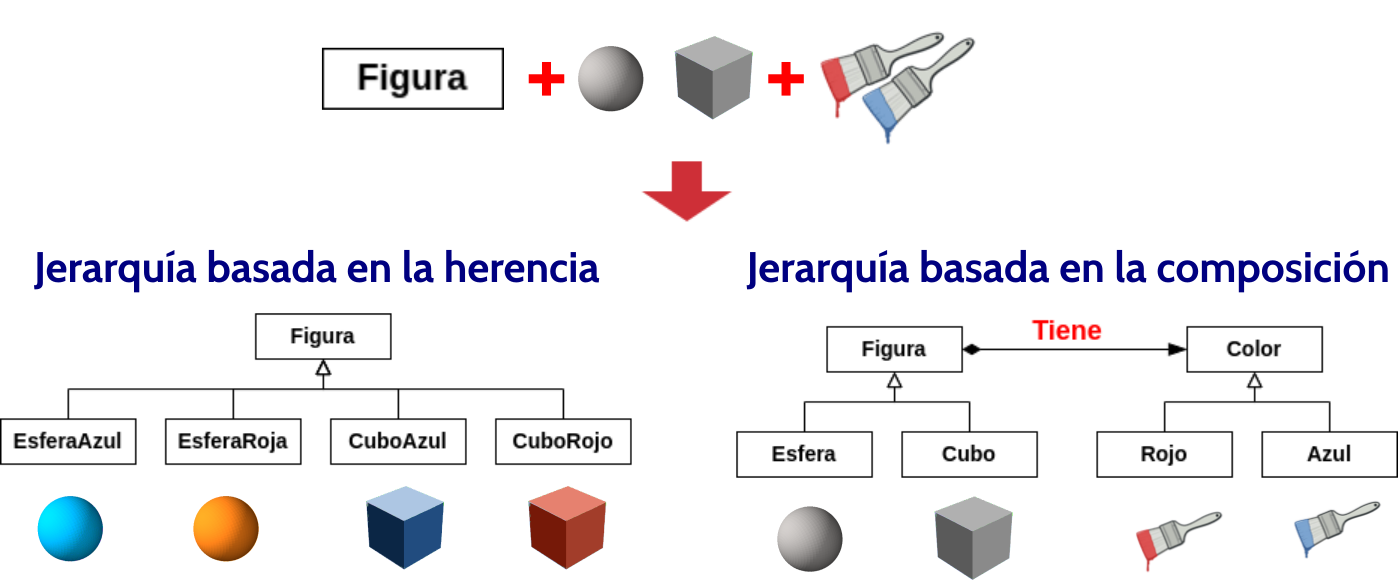
\includegraphics[width=\textwidth]{img/herencia_composicion.png}
      \caption{Diferentes jerarquías de clases según se priorice la herencia o la composición.}
      \label{fig_herencia_composicion}
   \end{center}
\end{figure}

En general, la composición da lugar a jerarquías de clases menos intrincadas, más sencillas de comprender y que se adaptan mejor a las pruebas, la depuración y las modificaciones.

Modelar el mundo a base de clases y objetos no deja de ser un tema subjetivo: cada programador puede encontrar diferentes formas de entender la jerarquía de categorías necesaria. De hecho, cada entidad de la vida real (\textit{clase}) puede servir para cosas muy diferentes (métodos de la clase). Por ejemplo, una taza puede servir para \textit{beber()}, pero también podría servir como arma (\textit{lanzar()}) o como \textit{pisapapeles()}.

Una de las reglas que se considera que debe cumplir cualquier diseño orientado a objetos es la \textit{encapsulación}, según la cual, el estado de los objetos no se debe poder modificar directamente desde fuera del objeto, sino solo a través de los métodos que proporciona la clase en cuestión. 

Por ejemplo, si se tuviera una clase denominada \textit{Etiqueta} con una propiedad llamada \textit{texto}, no se debería poder borrar el texto de la etiqueta mediante una instrucción del tipo:

{\centering \texttt{etiqueta.text = `` '';} \par}

Un diseño correcto proporcionaría un método \textit{borrar()} que realizase dicha acción de borrar el texto de la etiqueta:

{\centering \texttt{etiqueta.borrar();} \par}

Este procedimiento funciona perfectamente cuando las operaciones son sencillas, pero la cosa se complica cuando las acciones a realizar implican varios objetos de distintas clases. En esos casos, puede ser más sencillo utilizar funciones ajenas a las propias clases. Es una cuestión casi semántica: ¿en qué debemos poner más énfasis, en los sustantivos (\textit{Etiqueta}) o en los verbos (borrar()).

A medida que las jerarquías de clases crecen se hace cada vez más difícil preparar test que permitan probar los nuevos métodos que se implementan. Cada nuevo método necesita mucho trabajo de preparación para los test, y esta complejidad se incrementa de manera exponencial a medida que crece la jerarquía de clases.

Un planteamiento alternativo es que las clases prácticamente solo tengan datos y que las funciones que se necesiten para operar sobre esos datos sean externas a las clases. Esta técnica da lugar a una organización del código mucho más sencilla. Cada función solo realiza una tarea y cuando se quieren hacer test, solo hay que crear algunos juegos de datos de prueba y probar la función concreta, sin tener que luchar con una gran colección de clases y ficheros. Un caso típico donde este planteamiento es muy útil es cuando se trabaja con bases de datos relacionales, que se adaptan mal a la modelización de la POO.

Es ahí donde entran en juego las técnicas que proporciona la Programación Funcional (PF). Mientras que la Programación Orientada a Objetos se centra en la interacción y la comunicación entre diferentes objetos, la programación funcional se centra en cómo se van transformando los objetos. 

Dicha transformación hay que entenderla en el sentido de que un objeto se le pasa como argumento a una función que devuelve un nuevo objeto que incorpora las transformación que se quieren realizar. El objeto que devuelve la función es un nuevo objeto y el objeto original se puede conservar o desechar. En la programación funcional, unos objetos se transforman en otros, no se modifican.

\vfill\null

Se resumen a continuación algunas de las características de la programación orientada a objetos (POO):
\begin{itemize}
   \item \textbf{Estado de los objetos:} la POO está basada en objetos que encapsulan en una sola entidad su estado (propiedades) y su comportamiento (métodos). La \textit{mutabilidad} es una parte inherente de la POO. El estado de los objetos puede variar a lo largo del tiempo, lo que se consigue a través de los métodos que proporcionan las clases. De esta manera, se modelizan las entidades reales y sus relaciones. Esta mutabilidad es una forma natural de representar las propiedades de los objetos que necesitan cambiar de valor a lo largo del tiempo, pero da lugar a problemas complejos para gestionar estados globales y secundarios, por ejemplo en la programación concurrente.
   \item \textbf{Clases y herencia entre tipos:} la POO se basa en el concepto de clases como modelos de los objetos y a menudo utiliza la herencia entre clases para compartir y ampliar el comportamiento de las mismas.
   \item \textbf{Polimorfismo:} objetos de diferentes clases pueden ser tratados como si fueran de una misma clase base de la cual todos derivan.
   \item \textbf{Paradigma imperativo:} en general, la POO utiliza código con un paradigma imperativo, describiendo los pasos que hay que dar para modificar el estado de los objetos.
\end{itemize}

En el caso de la programación funcional (PF), algunas características distintivas son:
\begin{itemize}
   \item \textbf{Funciones sin estado:} está basada en la utilización de funciones que no mantienen ningún estado y operan sobre datos inmutables. En ese sentido, la PF separa el estado de los objetos de su comportamiento. El estado se representa mediante estructuras de datos inmutables. El comportamiento se expresa a través de funciones que operan sobre dichos datos.
   \item \textbf{Funciones como objetos de primera clase:} las funciones son objetos de primera clase que se pueden utilizar como parámetros de otras funciones, se pueden devolver como resultados y se pueden asignar a variables. Las funciones se utilizan para modelizar abstracciones, encapsular comportamientos. Para conseguir procesamientos complejos se utiliza la composición de funciones.
   \item \textbf{Paradigma declarativo:} la PF utiliza una codificación más declarativa, expresando la lógica de lo qué se quiere hacer, sin describir el flujo de instrucciones para ello. 
\end{itemize}

La opinión del autor es que no hay que ser fundamentalista de ningún paradigma de programación. Hay que recordar el viejo dicho: ``\textit{al que la única herramienta que conoce es el martillo, todo le parecen clavos}''. Hay problemas que se adaptan mejor a unas técnicas de programación u otras. En muchas ocasiones, una combinación adecuada de las técnicas de la POO y de la PF será lo más adecuado. En todos los casos hay que analizar el problema que se trata de resolver y utilizar la combinación de técnicas que mejor se adapte al mismo.

